\documentclass{article}

% if you need to pass options to natbib, use, e.g.:
% \PassOptionsToPackage{numbers, compress}{natbib}
% before loading nips_2016
%
% to avoid loading the natbib package, add option nonatbib:
% \usepackage[nonatbib]{nips_2016}

\usepackage{nips_2016}

% to compile a camera-ready version, add the [final] option, e.g.:
% \usepackage[final]{nips_2016}

\usepackage[utf8]{inputenc} % allow utf-8 input
\usepackage[T1]{fontenc}    % use 8-bit T1 fonts
\usepackage{hyperref}       % hyperlinks
\usepackage{url}            % simple URL typesetting
\usepackage{booktabs}       % professional-quality tables
\usepackage{amsfonts}       % blackboard math symbols
\usepackage{nicefrac}       % compact symbols for 1/2, etc.
\usepackage{microtype}      % microtypography
\usepackage{amsmath}
\usepackage{listings}
\usepackage{graphicx}
\title{Analysis on Logistic and Softmax Regression Using MNIST Dataset}

% The \author macro works with any number of authors. There are two
% commands used to separate the names and addresses of multiple
% authors: \And and \AND.
%
% Using \And between authors leaves it to LaTeX to determine where to
% break the lines. Using \AND forces a line break at that point. So,
% if LaTeX puts 3 of 4 authors names on the first line, and the last
% on the second line, try using \AND instead of \And before the third
% author name.

\author{
  Chetan Gandotra\thanks{Use footnote for providing further
    information about author (webpage, alternative
    address)---\emph{not} for acknowledging funding agencies.} \\
  Department of Computer Science\\
  UC San Diego\\
  San Diego, CA 92093 \\
  \texttt{cgandotr@ucsd.edu} \\
}

\author{
  David S.~Hippocampus\thanks{Use footnote for providing further
    information about author (webpage, alternative
    address)---\emph{not} for acknowledging funding agencies.} \\
  Department of Computer Science\\
  Cranberry-Lemon University\\
  Pittsburgh, PA 15213 \\
  \texttt{hippo@cs.cranberry-lemon.edu} \\
  %% examples of more authors
  %% \And
  Chetan Gandotra \\
  UC San Diego \\
  9500 Gilman Drive \\
  \texttt{cgandotr@ucsd.edu} \\
  %% \AND
  %% Coauthor \\
  %% Affiliation \\
  %% Address \\
  %% \texttt{email} \\
  %% \And
  %% Coauthor \\
  %% Affiliation \\
  %% Address \\
  %% \texttt{email} \\
  %% \And
  %% Coauthor \\
  %% Affiliation \\
  %% Address \\
  %% \texttt{email} \\
}

\begin{document}
% \nipsfinalcopy is no longer used

\maketitle

\begin{abstract}
  This report discusses the first programming assignment of course CSE 253: Neural Networks and Pattern Recognition, its solutions and the inferences. MNIST dataset was used and the hand-written digits in it were classified using Logistic and Softmax Regressions. Under Logistic Regression, two-way classification was performed on specific digits (2's and 3's, 2's and 8's). An accuracy of more than 97\% was achieved on both of these subsets of data using Logistic Regression. For Softmax Regression, we performed a ten-way classification (for all digits from 0 to 9) and achieved an accuracy of 87.65\% on the test set.
\end{abstract}

\section{Derivation of Gradient for Logistic Regression}

\subsection{Introduction}

The problem statement here is to find the gradient of the cost function. The error function for the logistic regression follows from the negative log likelihood, which can be written as:
$$E(w) = - \sum_{n=1}^{N} \{ t^{n} \ln y^{n} + ( 1-t^{n}) \ln(1-y^n)\}$$

\subsection{Methodology}

In this section, we will derive the gradient of cost function, which will be used in the later parts of this report. To find the optimal weight parameters, we need to take the partial derivative of the error function with respect to $w_{j}$ as follows:
$$\frac{\partial E(w)}{\partial w_j} = - \sum_{n=1}^{N} \left[ t^{n} \frac{\partial \ln y^{n}}{\partial w_j} + ( 1-t^{n}) \frac{\partial \ln(1-y^n)}{\partial w_j}\right]$$

$$\frac{\partial E(w)}{\partial w_j} = - \sum_{n=1}^{N} \left[ \frac{t^{n}}{y^{n}} \frac{\partial y^{n}}{\partial w_j} + \frac{( 1-t^{n})}{1-y^{n}} \frac{\partial (1-y^n)}{\partial w_j}\right]$$

Since $y^{n} = \sigma(\mathbf{w.x^{n}})$, the derivative can be written as:
$$\frac{\partial E(w)}{\partial w_j} = - \sum_{n=1}^{N} \left[ \frac{t^{n}}{\sigma(\mathbf{w.x^{n}})} \frac{\partial \sigma(\mathbf{w.x^{n}})}{\partial w_j} + \frac{( 1-t^{n})}{1-\sigma(\mathbf{w.x^{n}})} \frac{\partial ( 1-\sigma(\mathbf{w.x^{n}}))} {\partial w_j}\right]$$

Using the following properties of sigmoid function
\begin{align}
\sigma(-\mathbf{x}) = 1 - \sigma(\mathbf{x})	\\
\frac{\partial \sigma(-\mathbf{x})}{\partial x} = \sigma(\mathbf{x}) \sigma(-\mathbf{x})
\end{align}
the derivative can be written as:
$$\frac{\partial E(w)}{\partial w_j} = - \sum_{n=1}^{N} \left[ \frac{t^{n}}{\sigma(\mathbf{w.x^{n}})} \sigma(\mathbf{w.x^{n}}) \sigma(-\mathbf{w.x^{n}}) x_{j}^{n}  - \frac{( 1-t^{n})}{\sigma(-\mathbf{w.x^{n}})} \sigma(-\mathbf{w.x^{n}}) \sigma(\mathbf{w.x^{n}}) x_{j}^{n} \right]$$

$$\frac{\partial E(w)}{\partial w_j} = - \sum_{n=1}^{N} x_{j}^{n} \left[ t^{n} \sigma(-\mathbf{w.x^{n}})   - ( 1-t^{n}) \sigma(\mathbf{w.x^{n}}) \right]$$

Using (1) we get,
$$\frac{\partial E(w)}{\partial w_j} = - \sum_{n=1}^{N} x_{j}^{n} \left[ t^{n} (1-\sigma(\mathbf{w.x^{n}}))   - ( 1-t^{n}) \sigma(\mathbf{w.x^{n}}) \right]$$

Solving the above equation, we get:
$$\frac{\partial E(w)}{\partial w_j} = - \sum_{n=1}^{N} x_{j}^{n} \left[ t^{n} - \sigma(\mathbf{w.x^{n}}) \right]$$
or
$$-\frac{\partial E(w)}{\partial w_j} = \sum_{n=1}^{N} (t^{n} - y^{n}) x_{j}^{n}$$

\subsection{Results}

Hence, from the above derivation, it follows that for $n^{th}$ sample, the gradient of error can be written as:
$$-\frac{\partial E^{n}(w)}{\partial w_j} = (t^{n} - y^{n}) x_{j}^{n}$$

\subsection{Discussion}
The expression takes the difference between true label and predicted label and weigh it by the input data value. It makes sense because if there is a stark difference between the true and the predicted labels, the gradient value would be large. Thus, the corresponding component of the weight vector would be adjusted quickly in the direction of gradient to reduce the loss.

\newpage
\section{Derivation of Gradient for Softmax Regression}

\subsection{Introduction}
In this section, the focus is to find the gradient of the loss function of Softmax Regression - \emph{E(w)}. The error function for the softmax regression follows from the negative log likelihood, which can be written as:
$$E(w) = - \sum_{n=1}^{N} \sum_{k^{'}=1}^{C} t_{k^{'}}^{n} \ln y_{k^{'}}^{n}$$

\subsection{Methodology}
To find the optimal weight parameters for each class, we need to take the partial derivative of the error function with respect to $w_{jk}$ as follows:
$$\frac{\partial E(w)}{\partial w_{jk}} = - \sum_{n=1}^{N} \sum_{k^{'}=1}^{C} \left[ t_{k^{'}}^{n} \frac{\partial \ln y_{k^{'}}^{n}}{\partial w_{jk}} \right]$$

\begin{align}
- \frac{\partial E(w)}{\partial w_{jk}} = \sum_{n=1}^{N} \left[ \frac{t_{k}^{n}}{y_{k}^{n}} \frac{\partial y_{k}^{n}}{\partial w_{jk}}\right] + \sum_{k^{'}\neq k} \left[ \frac{t_{k^{'}}^{n}}{y_{k^{'}}^{n}} \frac{\partial y_{k^{'}}^{n}}{\partial w_{jk}} \right]
\end{align}

Since, $$y_{k}^{n} = \frac{e^{\mathbf{w_{k}.x^{n}}}}{\sum_{l=1}^{C} e^{\mathbf{w_{l}.x^{n}}}}$$ the derivatives $\frac{\partial y_{k}^{n}}{\partial w_{jk}}$ and $\frac{\partial y_{k^{'}}^{n}}{\partial w_{jk}}$ can be written as:

$$\frac{\partial y_{k}^{n}}{\partial w_{jk}} = \frac{e^{\mathbf{w_{k}.x^{n}}}}{\sum_{l=1}^{C} e^{\mathbf{w_{l}.x^{n}}}} x^{n}_{j} - e^{\mathbf{w_{k}.x^{n}}} \left[ \frac{1}{(\sum_{l=1}^{C} e^{\mathbf{w_{l}.x^{n}}})^{2}} \right] e^{\mathbf{w_{k}.x^{n}}} x^{n}_{j}$$

\begin{align}
\frac{\partial y_{k}^{n}}{\partial w_{jk}} = \left(y_{k}^{n} - (y_{k}^{n})^{2}\right) x^{n}_{j}
\end{align}

$$\frac{\partial y_{k^{'}}^{n}}{\partial w_{jk}} = - e^{\mathbf{w_{k^{'}}.x^{n}}} \left[ \frac{1}{(\sum_{l=1}^{C} e^{\mathbf{w_{l}.x^{n}}})^{2}} \right] e^{\mathbf{w_{k^{'}}.x^{n}}} x^{n}_{j}$$

\begin{align}
\frac{\partial y_{k^{'}}^{n}}{\partial w_{jk}} = - \left(y_{k^{'}}^{n}\right)^{2} x^{n}_{j}
\end{align}

Substituting (4) and (5) in (3), we get

$$- \frac{\partial E(w)}{\partial w_{jk}} = \sum_{n=1}^{N} \left[ \frac{t_{k}^{n}}{y_{k}^{n}} \left(y_{k}^{n} - (y_{k}^{n})^{2}\right) x^{n}_{j} \right] - \sum_{k^{'}\neq k} \left[ \frac{t_{k^{'}}^{n}}{y_{k^{'}}^{n}} \left(y_{k^{'}}^{n}\right)^{2} x^{n}_{j} \right]$$

\begin{align}
- \frac{\partial E(w)}{\partial w_{jk}} = \sum_{n=1}^{N} \left[ t_{k}^{n}\left(1 - y_{k}^{n}\right) x^{n}_{j} \right] - \sum_{k^{'}\neq k} \left[ t_{k^{'}}^{n} y_{k^{'}}^{n} x^{n}_{j} \right]
\end{align}

Now, for any sample, only one of the C labels in $t^{n}$ would be 1, and all the others would be 0. This is because the label one would be the label set, and each training example can correspond to only one label.
Thus, for any sample $a$ where $t^{n}_{k}$ is 1, the derivative would be:

$$- \frac{\partial E^{a}(w)}{\partial w_{jk}} = \left[ \left(1 - y_{k}^{a}\right) x^{a}_{j} \right]$$
or it could be written as:
\begin{align}
- \frac{\partial E^{a}(w)}{\partial w_{jk}} = \left[ \left(t^{n}_{k} - y_{k}^{a}\right) x^{a}_{j} \right]
\end{align}

For any sample $b$ where one of $t^{n}_{k^{'}}$ is 1 (where $k^{'} \neq k$), the derivative would be:
$$- \frac{\partial E^{b}(w)}{\partial w_{jk}} = \left[ \left(- y_{k}^{b}\right) x^{b}_{j} \right]$$ 
or it could be written as:
\begin{align}
- \frac{\partial E^{b}(w)}{\partial w_{jk}} = \left[ \left(t^{n}_{k} - y_{k}^{b}\right) x^{b}_{j} \right]
\end{align}

Using the results of (7) and (8), (6) could be written as:

$$- \frac{\partial E(w)}{\partial w_{jk}} = \sum_{n=1}^{N} \left( t_{k}^{n} - y_{k}^{n}\right) x^{n}_{j}$$

\subsection{Results}
Thus, using our findings above, we can say that for $n^{th}$ sample, the derivative can be written as:
\begin{align}
- \frac{\partial E^{n}(w)}{\partial w_{jk}} = \left( t_{k}^{n} - y_{k}^{n}\right) x^{n}_{j}
\end{align}

\subsection{Discussion}
Interestingly, the expression of gradient looks similar to that of logistic regression. In this case, the derivative takes the difference between true label and predicted label for the $k^{th}$ class and weigh it by the input data value. Again, if the difference is big between the true and the predicted labels, the gradient value would be large. Thus, the corresponding component of the weight vector would be adjusted quickly in the direction of gradient to reduce the loss.

\newpage
\section{Read in Data}

\subsection{Introduction}
As mentioned in the abstract, we deal with the "MNIST" dataset in this programming assignment. The first and foremost task before operating on the data was to load it. 

\subsection{Methodology}
The MNIST data was downloaded from the website at \emph{http://yann.lecun.com/exdb/mnist/} (the same link as given in PA1). To read the data, GitHub library at \emph{https://github.com/akosiorek/CSE/blob/master/MLCV/} was used, which returns the training and testing data in matrix form, and labels as a vectors. Operations were then performed on this data to add a column of ones (bias term) at the beginning and to extract digit specific data (2-3's and 2-8's). Also, the data was restricted to first 20k entries, 10\% of which was allocated to a hold-out set. The size of test data was kept as two thousand. This was done by picking the first 2k entries from the test data returned by the library.

\subsection{Results}
Using some existing libraries on Github, we were able to extract the data into variables in Python. This data, however, consisted of the full 60k training data points and 10k testing data points. We extracted the first 20k training data points and the first 2k testing data points. 10\% of the training data was designated as a hold-out set.

\subsection{Discussion}
Computation on large data sets can often be time consuming. Due to this reason, we extracted the full data and restricted the size of training, validation and test sets. This allowed faster computations throughout the programming assignment. A hold-out set acts as a dummy test set, which we use so as to improve performance of our model by testing it on the hold-out set. Good accuracy on hold-out set leads to a good accuracy on test set in general. 

\section{Logistic Regression via gradient descent}

\subsection{Introduction}
In this part, we are required to use logistic regression and classify a given hand-written digit as either 2 or 3. Since logistic regression uses binary output, we say that the target is 1 if the input is from the "2" category and 0 if it is from the other category. We are required to produce the following:
\begin{enumerate}
  \item Plot of loss function (\emph{E}) over the training set, test set and the hold-out set
  \item Plot of percent correct classification over training for the training set, the hold-out set, and the test set
  \item The above two plots for digits 2 and 8
  \item Display weights as images for both the classifiers (2 vs. 3 and 2 vs. 8). Plot the difference between weights as well.
\end{enumerate}

\subsection{Methodology}
To plot the first graph, loss function is put against the Y-axis, and the iteration number along the X-axis. The loss function used was:
$$E(w) = - \sum_{n=1}^{N} \{ t^{n} \ln y^{n} + ( 1-t^{n}) \ln(1-y^n)\}$$
This was done for all the three sets - training, test and validation. Hence, for each set, the value of \emph{N} and the corresponding data/labels change. This procedure was repeated for the 2's and 8's data set.

In the next graph, we plotted "percent correct" against the iteration number. The value of percent correct can be inferred by going over all the examples as test set in a way, and seeing what our model predicts on it. For every correct classification, we add one to the number of data points classified correctly. Then, at the end, we find the corresponding percentage. This is repeated at each iteration for all the three sets - training, test and validation. Again, this procedure was repeated for the 2's and 8's data set.

To display the weight vectors for both the cases and their difference, the bias term in them was dropped. This reduced the weight vector to a 784 dimensional vector, which was re-shaped into a 28 x 28 matrix and then plotted using Python.

\subsection{Results}

Various results we got are plotted follows:

\begin{figure}[h!]
  \centering
  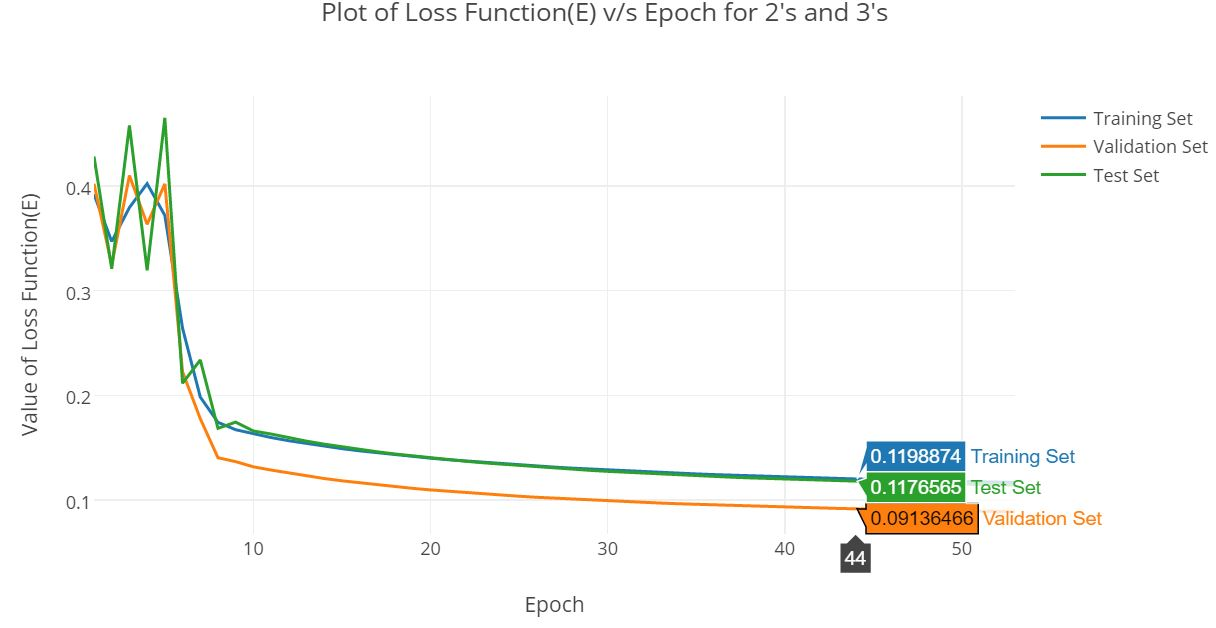
\includegraphics[width=\linewidth]{graphs/4a_23.JPG}
  \caption{Loss Function (E) vs Epoch for 2's and 3's}
  \label{fig:graph 4(a)_23}
\end{figure}

\begin{figure}[h!]
  \centering
  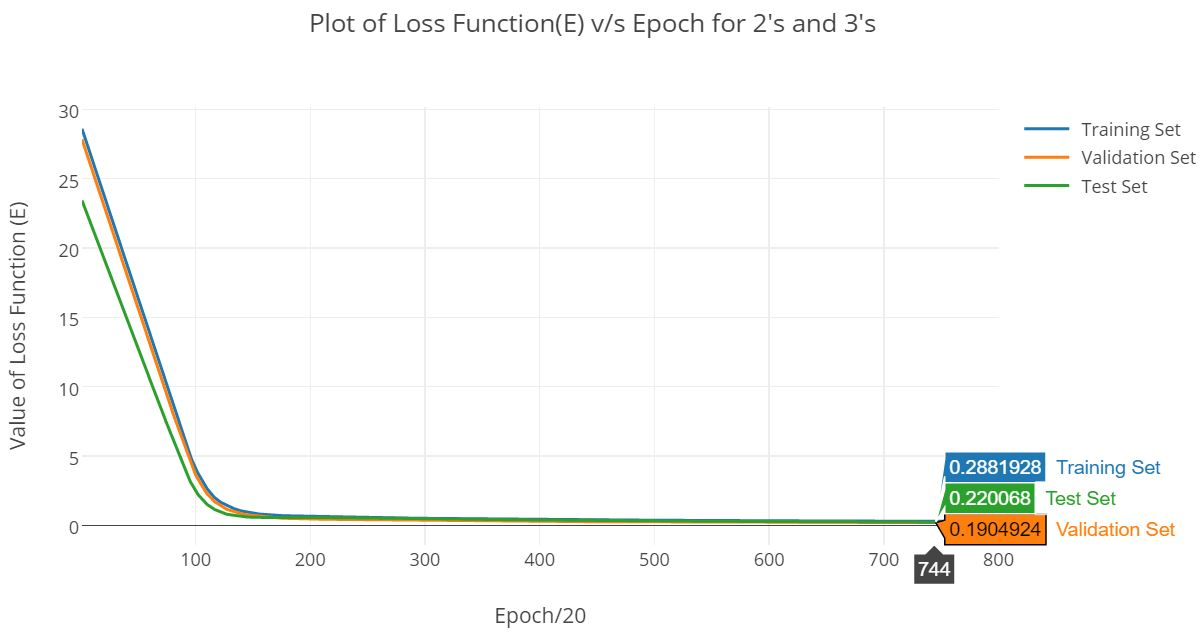
\includegraphics[width=\linewidth]{graphs/4a.JPG}
  \caption{Loss Function calculated every 1/20 of Epoch vs Epoch for 2's and 3's}
    \label{fig:graph 4(a)_batch_23}
\end{figure}

\begin{figure}[h!]
  \centering
  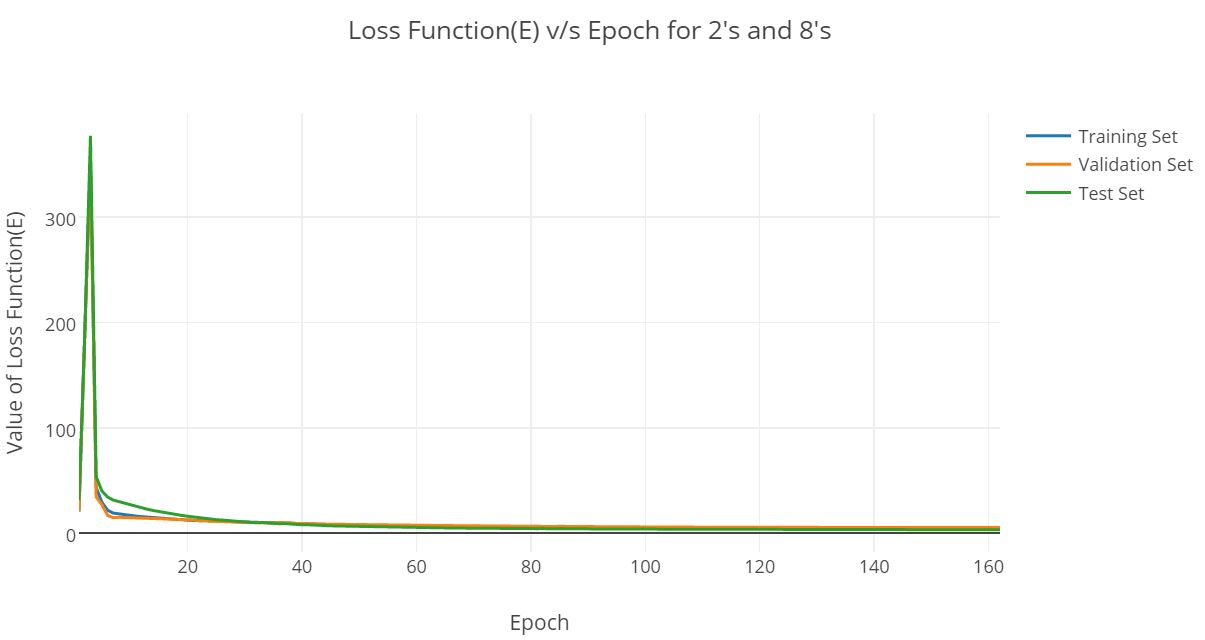
\includegraphics[width=113mm]{graphs/4a_28.JPG}
  \caption{Loss Function (E) vs Epoch for 2's and 8's}
    \label{fig:graph 4(a)_28}
\end{figure}

\begin{figure}[h!]
  \centering
  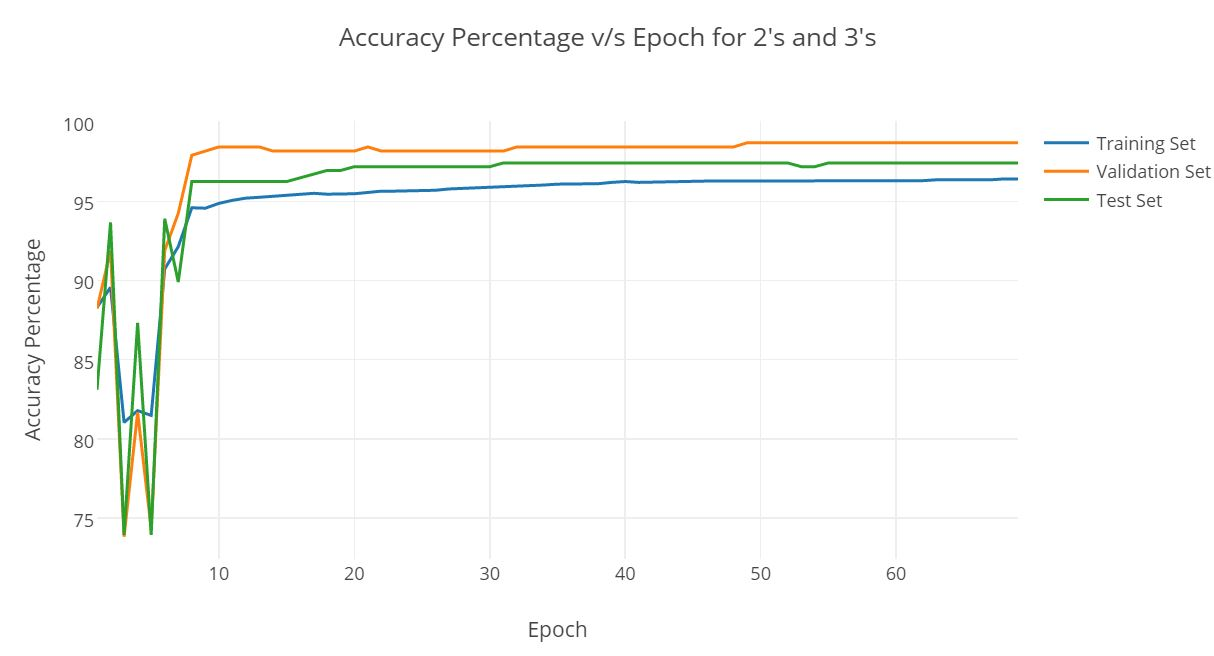
\includegraphics[width=113mm]{graphs/4b_23.JPG}
  \caption{Percent correct classification vs Epoch for 2's and 3's}
  \label{fig4}
\end{figure}

\begin{figure}[h!]
  \centering
  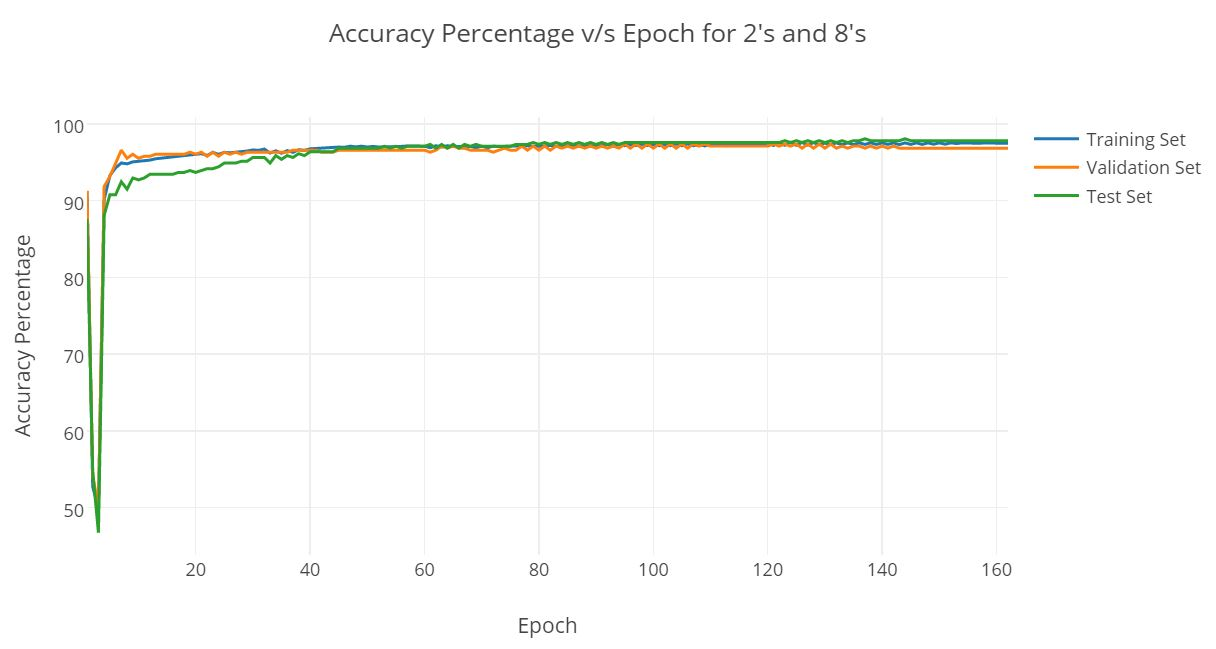
\includegraphics[width=113mm]{graphs/4b_28.JPG}
  \caption{Percent correct classification vs Epoch for 2's and 8's}
  \label{fig5}
\end{figure}

\begin{figure}[h!]
  \centering
  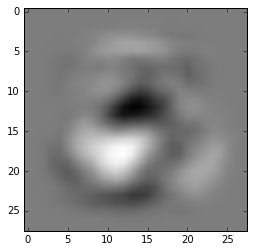
\includegraphics[width=35mm, scale=0.4]{graphs/23WeightsImage.png}
  \caption{Weights as an image for 2's and 3's}
   \label{fig6}
\end{figure}

\begin{figure}[h!]
  \centering
  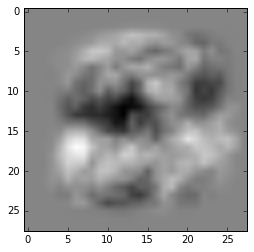
\includegraphics[width=35mm, scale=0.4]{graphs/28WeightsImage.png}
  \caption{Weights as an image for 2's and 8's}
    \label{fig7}
\end{figure}

\begin{figure}[h!]
  \centering
  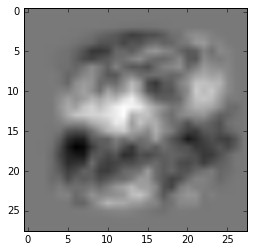
\includegraphics[width=35mm, scale=0.4]{graphs/DifferenceWeightsImageNoReg23_28.png}
  \caption{Difference of weights as an image for 2's and 3's and 2's and 8's}
    \label{fig8}
\end{figure}


\subsection{Discussion}

Generally, we assume that the data for training and testing are generated from same underlying distribution. Thus, they have similar underlying properties. However, since test data is not available to us in the real world, we extract a portion of training data to test our model and call it a validation set. And since, validation set and test set are generated from the same underlying distribution, the performance of our model should not vary much on validation and test set in ideal case (it would very a little bit in our case as validation set is small as compared to test set). The aforementioned behavior is reaffirmed by our experiments. From figure \ref{fig:graph 4(a)_23} and figure \ref{fig:graph 4(a)_batch_23}, we see that curves for validation error and test error are similar and validation error hovers around the test error. Same is the case for classification of 2's and 8's in figure \ref{fig:graph 4(a)_28}. Thus, we can safely say that validation set closely captures how our model would perform on test data. One interesting thing to note is that in the case of batching (contained 1/20 of all points), the curve of error function is smooth . This is because the gradient is calculated only on few points at a time, which makes the gradient increase gradually towards the optimum. 

We have chosen the value of the hyperparameter T as 2000 empirically. Also, for the early stopping of our algorithm, we have checked whether the error is non-decreasing on 15 iterations. The reason for choosing a bit large value is that the error on the validation set used to change in the steps of 5-10 iterations. Thus, just to insure that the error does not decrease after early stopping, we took added some buffer iterations. 

In figure \ref{fig4} and figure \ref{fig5}, we see that the accuracy percentage increases over time. This is expected, as with more number of iterations, we minimize loss and fit the data. This means that we will be able to classify more number of points correctly leading to higher accuracy. Also, note that the graph of 2's and 8's is more overlapping. This can be because the validation/test data is very similar to the training data.

Next, we plot the weight vectors for three cases - 2's and 3's, 2's and 8's, and the difference of these two in figure \ref{fig6}, \ref{fig7} and\ref{fig8} respectively. For both 2's and 3's case and the 2's and 8's case, the weight vector seems like images of 2 and 8 have been superimposed. This seems intuitively correct as the weight vector needs to predict either of these. For the difference case, the image looks like a mirror-image of 3. This is because the 2's component is common in both the cases and must get cancelled out. Thereafter, we are left with 8's and 3's, which superimposition cancel out too. Hence, what we are left with is the portion of 8 that was not covered by 3 and thus looks like a mirror image of 3.


\newpage
\section{Regularization}

\subsection{Introduction}

Regularization is a commonly used technique to improve the model generalization. We write the regularized loss function \emph{J(w)} as:

$$J(w) = E(w) + \lambda C(w)$$

where \emph{C(w)} is the complexity penalty and $\lambda$ is the strength of regularization. For $\lambda$ = 0, \emph{J} reduces to \emph{E}. Considering $L_{2}$ norm as the complexity penalty, we have:

$$J(w) = E(w) + \lambda ||w||^2$$

For $L_{1}$ norm, we have:

$$J(w) = E(w) + \lambda |w|$$

In the first part, we are expected to derive the update term for both $L_{1}$ and $L_{2}$ penalties.

Next, we are expected to plot the percent correct v/s iterations graph for different $\lambda$ values. This is followed by plotting length of weight vector v/s iterations for different $\lambda$ values. Then, we plot the final test error with each of the $\lambda$. Finally, we are expected to plot the weights as images.

\subsection{Methodology}

To derive the update term, we take derivative of this function with respect to \emph{w}, the weight vector. Hence, we have:

$$\frac{\partial J(w)}{\partial w} = \frac{\partial E(w)}{\partial w} + \lambda\frac{\partial C(w)}{\partial w}$$

We have already calculate the first part of the equation - $\frac{\partial E(w)}{\partial w}$ in Question 1. Hence, according to the question, solving for $\frac{\partial C(w)}{\partial w}$, we have:

$$\frac{\partial C(w)}{\partial w} = \frac{||w||^2}{\partial w} = 2w$$

Therefore, we have:
$$\frac{\partial J(w)}{\partial w} = \frac{\partial E(w)}{\partial w} + 2\lambda w$$

Similarly, for $L_{1}$ norm as the complexity penalty, we have 
$$J(w) = E(w) + \lambda |w|$$
Therefore, 
$$\frac{\partial J(w)}{\partial w} = \frac{\partial E(w)}{\partial w} + \frac{\partial \lambda |w|}{\partial w}$$

$$\frac{\partial J(w)}{\partial w} = \frac{\partial E(w)}{\partial w} + \lambda \frac{\partial |w|}{\partial w}$$

Now, the entry at index \emph{j} of partial derivative of \emph{|w|} can be written as: 

\[
	\frac{\partial |w|}{\partial w_j} = \left\{
                \begin{array}{ll}
                  1, if w_j \geq 0\\
                  -1, otherwise
                \end{array}
              \right.
\]

Thus, the value of $\frac{\partial |w|}{\partial w}$ is A vector of all one's or minues one's depending upon the sign of entries in \emph(w) vector and has the same number of elements as in \emph{w}.

To plot the graphs, a similar approach as in Section 4 was undertaken. The only difference was that earlier we did it for different data sets - training, test and validation. In these graphs, we always take the training set and calculate percent error and length of weight vector at that iteration. This is done multiple times by changing $\lambda$ values. Then, we plot the final test error for each $\lambda$ value, keeping the learning rate fixed. This plot is made as a bar graph, with one bar for each $\lambda$. Finally, we plot the weights as images like we did in Section 4. To display the weight vectors, the bias term was dropped. This reduced the weight vector to a 784 dimensional vector, which was re-shaped into a 28 x 28 matrix and then plotted using Python.

\subsection{Results}
The partial derivative of loss function with $L_{1}$ norm regularization is:
$$\frac{\partial J(w)}{\partial w} = \frac{\partial E(w)}{\partial w} + \lambda \frac{\partial |w|}{\partial w}$$

where the partial derivative of \emph{|w|} can be written as: 

\[
	\frac{\partial |w|}{\partial w_j} = \left\{
                \begin{array}{ll}
                  1, if w_j \geq 0\\
                  -1, otherwise
                \end{array}
              \right.
\]

and the partial derivative in case of $L_{2}$ norm regularization is:

$$\frac{\partial J(w)}{\partial w} = \frac{\partial E(w)}{\partial w} + 2\lambda w$$

The "percent correct" value was plotted over the number of training iterations for the training set, for different lambda values keeping the other hyper-parameters same. 

Parameters used: \textbf{Penalty} = $L_{2}$ norm, \textbf{Learning rate} $\eta$ = 0.0001

\begin{figure}[h]
  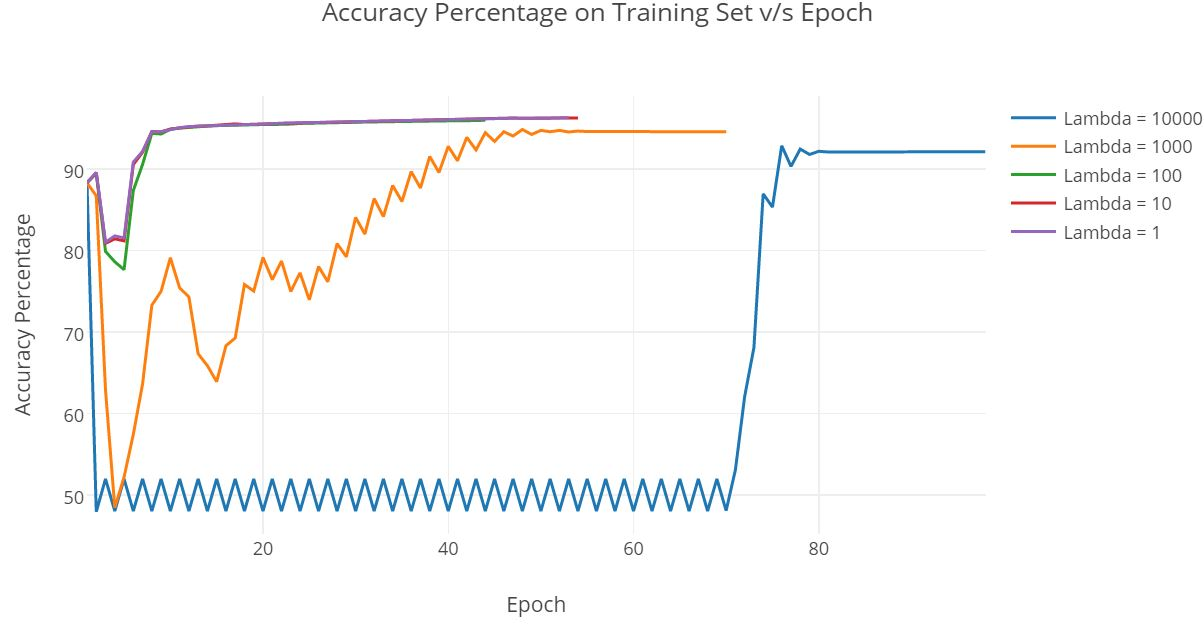
\includegraphics[width=\linewidth]{graphs/5_b_negativeInEqn.JPG}
  \caption{Accuracy Percentage v/s Epoch for $L_{2}$ norm}
  \label{fig:graph 5(b) l2}
\end{figure}


Now for penalty as $L_{1}$ norm and Learning rate $\eta$ = 0.0001, we have:
\newpage
\begin{figure}[t]
  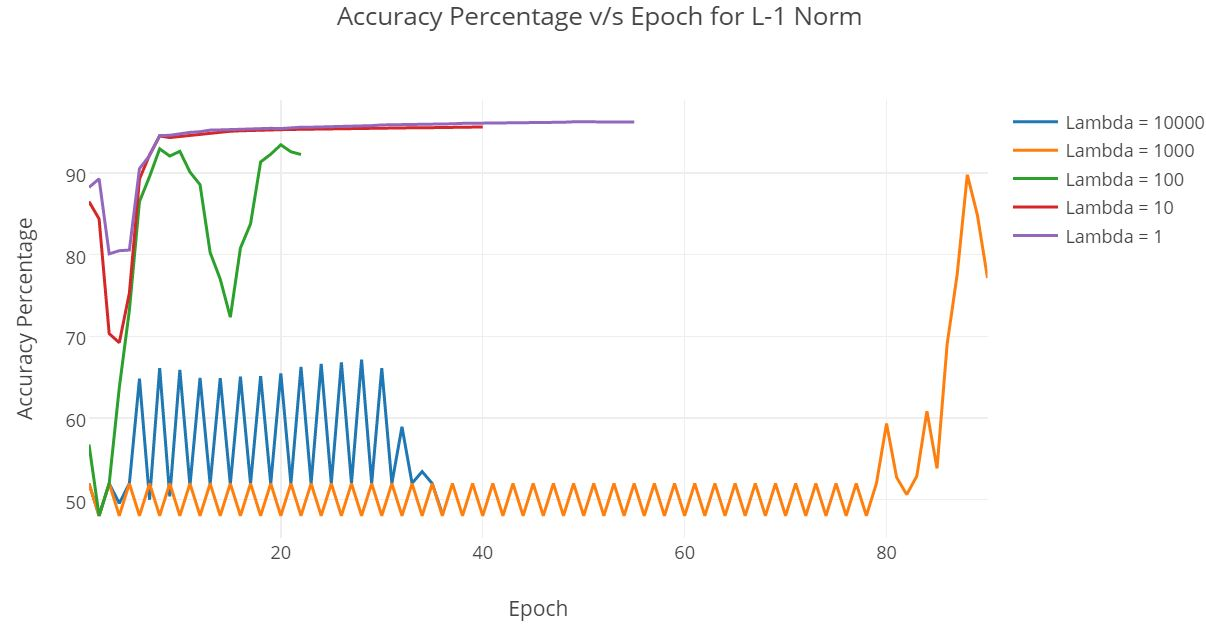
\includegraphics[width=105mm]{graphs/5_b_L1_new.JPG}
  \caption{Accuracy Percentage v/s Epoch for $L_{1}$ norm}
  \label{fig:graph 5(b) l1}
\end{figure}
The length of weight vector against training iterations produced a graph as follows for the $L_{2}$ norm case:
\begin{figure}[h!]
  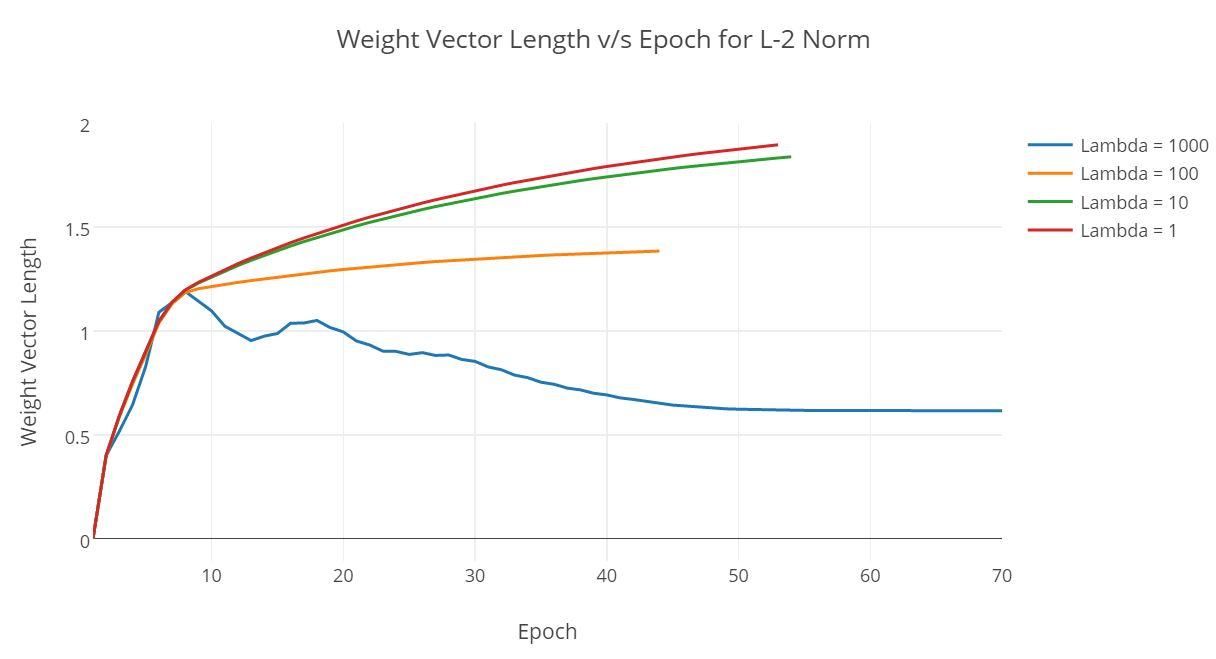
\includegraphics[width=105mm]{graphs/5_c.JPG}
  \caption{Weight Vector Length v/s Epoch with $L_{2}$ norm}
  \label{fig:graph 5(c) l2}
\end{figure}

For $L_{1}$ norm, it becomes:
\begin{figure}[h!]
  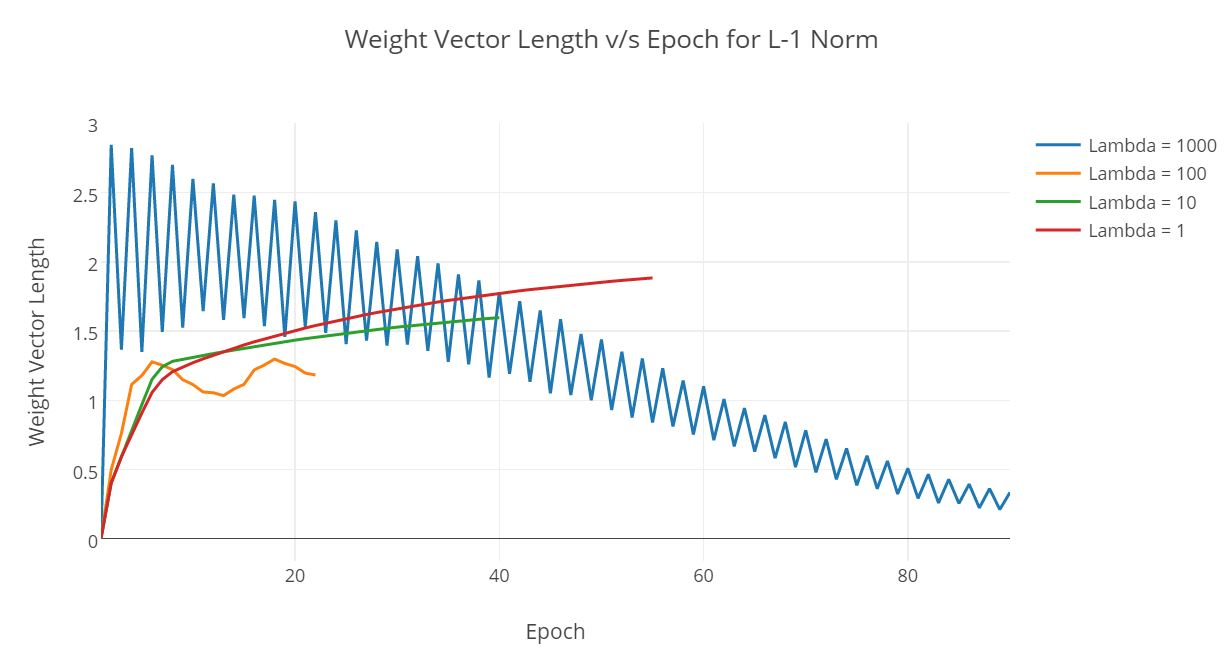
\includegraphics[width=105mm]{graphs/5_c_negative_l1.JPG}
  \caption{Weight Vector Length v/s Epoch with $L_{1}$ norm}
  \label{fig:graph 5(c) l1}
\end{figure}

Note that the learning rate $\eta$ used was 0.0001 in both the cases.

The plot of final test error for various $\lambda$ values with $L_{2}$ norm penalty is as follows:

\begin{figure}[h!]
  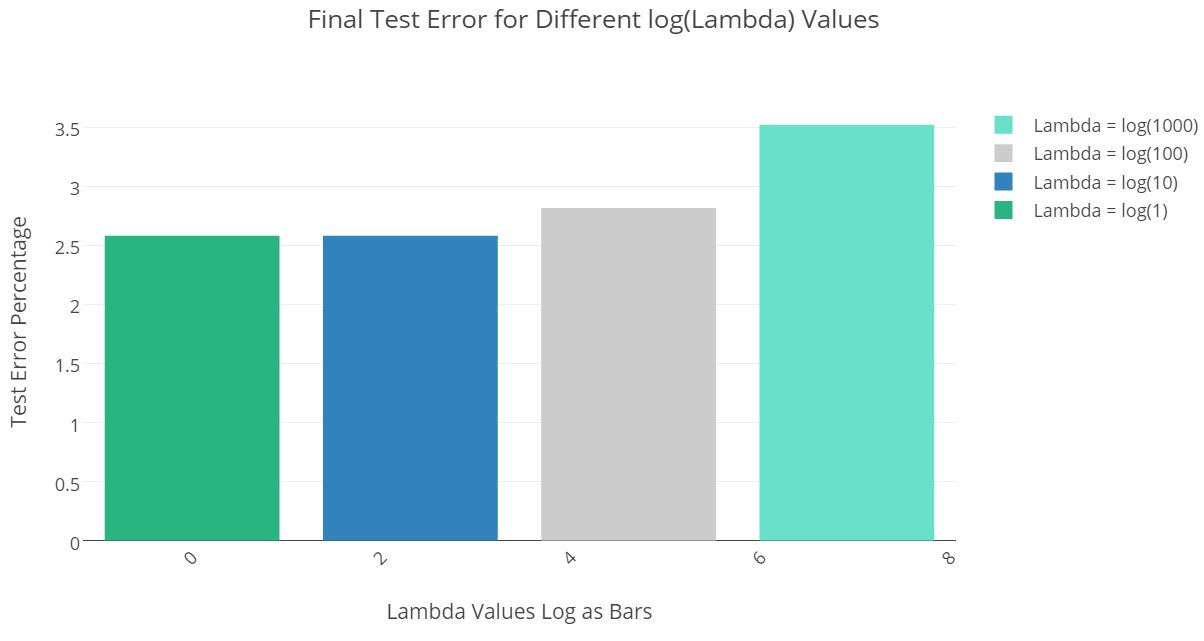
\includegraphics[width=\linewidth]{graphs/5_d_negative.JPG}
  \caption{Final Test Error v/s Log($\lambda$) $L_{2}$ norm}
  \label{fig:graph 5(d) l2}
\end{figure}

The plot of final test error for various $\lambda$ values with $L_{1}$ norm penalty is as follows:

\begin{figure}[h!]
  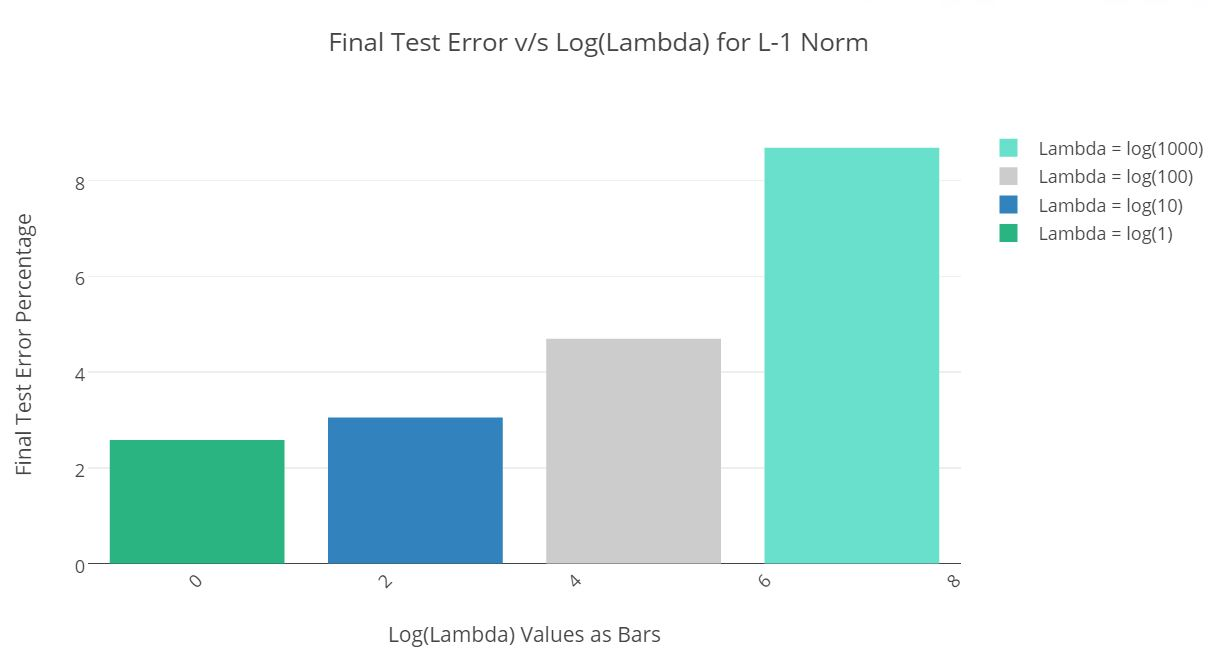
\includegraphics[width=\linewidth]{graphs/5_d_l1.JPG}
  \caption{Final Test Error v/s Log($\lambda$) $L_{1}$ norm}
  \label{fig:graph 5(d) l1}
\end{figure}

Note that the learning rate $\eta$ used was 0.0001 in both the cases.


For \textbf{L1} norm: using learning rate $\eta$ as 0.0001 in both the cases and different $\lambda$ values, the final weight vectors were plotted as images. Here are the findings:
\newpage
\begin{figure}[h!]
  \centering
  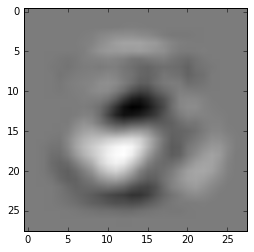
\includegraphics[width=40mm, scale=0.5]{graphs/23Weights_l1_1.PNG}
  \caption{Weight Vector Image for 2's and 3's with $L_{1}$ norm and $\lambda = 1$}
  \label{fig15}
\end{figure} 

\begin{figure}[h!]
    \centering
  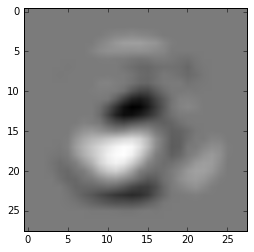
\includegraphics[width=40mm, scale=0.5]{graphs/23Weights_l1_10.PNG}
  \caption{Weight Vector Image for 2's and 3's with $L_{1}$ norm and $\lambda = 10$}
  \label{fig16}
\end{figure}

\begin{figure}[h!]
    \centering
  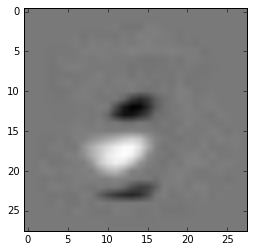
\includegraphics[width=40mm, scale=0.5]{graphs/23Weights_l1_100.PNG}
  \caption{Weight Vector Image for 2's and 3's with $L_{1}$ norm and $\lambda = 100$}
  \label{fig17}
\end{figure}

\begin{figure}[h!]
    \centering
  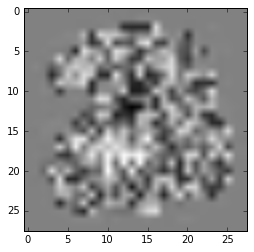
\includegraphics[width=40mm, scale=0.5]{graphs/23Weights_l1_1000.PNG}
  \caption{Weight Vector Image for 2's and 3's with $L_{1}$ norm and $\lambda = 1000$}
  \label{fig18}
\end{figure}

For \textbf{L1} norm: Using learning rate $\eta$ as 0.0001 in both the cases and optimal $\lambda$ value of 0.0001, the image looks like following:
\newpage
\begin{figure}[h!]
    \centering
  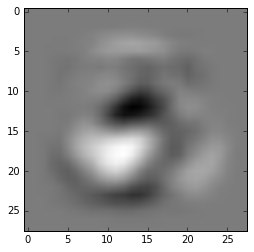
\includegraphics[width=40mm, scale=0.5]{graphs/23WeightsImage_Regularization.PNG}
  \caption{Weight Vector Image for 2's and 3's with $L_{1}$ norm and $\lambda = 0.0001$}
  \label{fig19}
\end{figure}


For \textbf{L2} norm: using learning rate $\eta$ as 0.0001 in both the cases and different $\lambda$ values, the final weight vectors were plotted as images. Here are the findings:

\begin{figure}[h!]
  \centering
  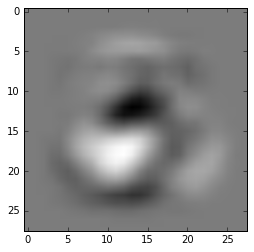
\includegraphics[width=40mm, scale=0.5]{graphs/23Weights_l2_1.PNG}
  \caption{Weight Vector Image for 2's and 3's with $L_{2}$ norm and $\lambda = 1$}
  \label{fig:graph 5(e) l2}
\end{figure} 

\begin{figure}[h!]
    \centering
  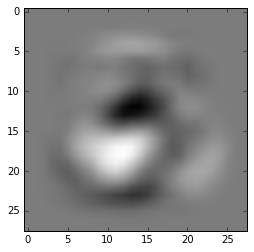
\includegraphics[width=40mm, scale=0.5]{graphs/23Weights_l2_10.PNG}
  \caption{Weight Vector Image for 2's and 3's with $L_{2}$ norm and $\lambda = 10$}
  \label{fig:graph 5(e) l1}
\end{figure}

\begin{figure}[h!]
    \centering
  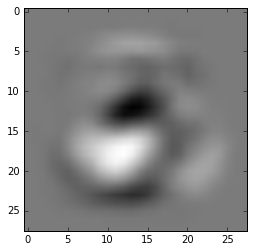
\includegraphics[width=40mm, scale=0.5]{graphs/23Weights_l2_100.PNG}
  \caption{Weight Vector Image for 2's and 3's with $L_{2}$ norm and $\lambda = 100$}
  \label{fig:graph 5(e) l1}
\end{figure}

\begin{figure}[h!]
    \centering
  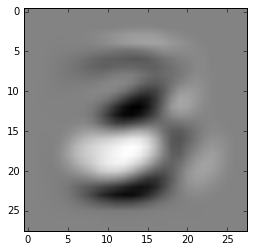
\includegraphics[width=40mm, scale=0.5]{graphs/23Weights_l2_1000.PNG}
  \caption{Weight Vector Image for 2's and 3's with $L_{2}$ norm and $\lambda = 1000$}
  \label{fig:graph 5(e) l1}
\end{figure}
\newpage
For \textbf{L2} norm: Using learning rate $\eta$ as 0.0001 in both the cases and optimal $\lambda$ value of 0.0001, the image looks like following:

\begin{figure}[h!]
    \centering
  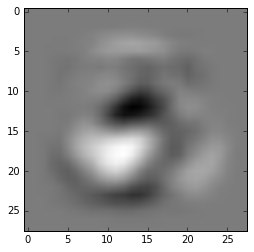
\includegraphics[width=40mm, scale=0.5]{graphs/23WeightsImage_Regularization.PNG}
  \caption{Weight Vector Image for 2's and 3's with $L_{2}$ norm and $\lambda = 0.0001$}
  \label{fig:graph 5(e) l1}
\end{figure}


\subsection{Discussion}

Note that the $L_{1}$ norm is not differentiable at 0. However, all that matters is that we can compute a subgradient / subderivative. Since it's differentiable everywhere else, we can just fill in any "reasonable"value (such as -1 or 1; we have chosen -1) for the gradient at 0. So, for the cases where the weights are negative, we would have positive regularization term that would drive them towards zero and for the cases where the weights are positive, the regularization term would be negative, thus decreasing the weights. Hence, $L_{1}$ tries to limit the coefficient which restricts overfitting.

Graph \ref{fig:graph 5(b) l2} shows how the accuracy on training data varies according to the iteration number (epoch) for several $\lambda$ values. $\lambda$ is added to avoid over-fitting. Thus, higher the $\lambda$ value, lower will be the accuracy on training set as more emphasis is given to the complexity function rather than the original loss function \emph{E(w)}. 

Graph \ref{fig:graph 5(b) l1} shows how the accuracy on training data varies according to the iteration number (epoch) for several $\lambda$ values. The same generalization as above holds here as well. Note that the graph line for $\lambda$ = 10000 overlaps with that of $\lambda$ = 1000 and is not visible clearly.

Next, we plot the length of weight vectors against training iterations for different $\lambda$ values. In both the cases, as $\lambda$ increases, the corresponding weight vector length value decreases. Both these values are inversely related. This is due because as $\lambda$ increases, the overall regularized loss function value tends to increase. However, since our goal is to minimize loss, the weight vector balances this increase in $\lambda$ by decreasing itself. A similar argument is valid for decreasing $\lambda$ values as well.

Then we have the plots of final test error for different log($\lambda$) values. In both the above graphs, as $\lambda$ (or log($\lambda$)) increases, the final test error increases. This is because for large $\lambda$ values, the model complexity is low. Beyond a certain level, the complexity may become so low that it no longer fits the data well leading to mis-classification on a large number of points. Increasing $\lambda$ value only decreases the complexity further, leading to even further decline in test accuracy. Similarly, if the $\lambda$ value is too low, the model may become highly complex, so much so that over-fitting happens. Test error in this case will again be large, as the model won't generalize well for points in test set.

Finally, we have the weight vector images. Since, regularization limits the weights from being too high, the images of weights are little bit softer in nature.

\newpage
\section{Softmax Regression Via Gradient Descent}

\subsection{Introduction}
The task at hand is to perform Softmax Regression on the MNIST data set and come up with the best parameters that may perform well on the test data, without actually looking at test data. Then, we need to plot the loss function values over number of training iterations for training, hold-out and test data sets. Finally, we are expected to plot the percent correct values over training iterations the three data set parts. 

\subsection{Methodology}
Softmax Regression was performed on the first 20,000 training data points and was used to do a 10-way classification of the hand-written digits using a hold-out set and regularization parameter $\lambda$. The size of hold-out set was again set to 10\% of the size of training data. To figure out the best hyper-parameter values, a hold-out set was used. The parameters performing the best on this hold-out set were chosen to be the final parameters. The loss function(E) was plotted over the number of training iterations for the training, hold-out and test sets. 

Parameters used:
Penalty = $L_{2}$ norm;
Regularization parameter $\lambda$ = 0.0001;
Learning rate $\eta$ = 0.0001

Next, the "percent correct" (or accuracy percentage) was plotted over the number of training iterations for the training, hold-out and test sets. Same parameters as above were used.

\subsection{Results}
The percentage error values recorded on the hold-out set for different values of hyper-parameters are as follows:

\begin{table}[h!]
  \caption{Error on Hold-out Set for Different Hyper-parameters}
  \label{table1}
  \centering
  \begin{tabular}{llll}
    \toprule
    $\eta$     & $\lambda$     & Norm     & Error \% \\
    \midrule
    0.0001     & 0.01     & L-1/L-2     & 8.1  \\
    0.0001     & 0.1     & L-1/L-2     & 8.1     \\
    0.0001     & 0.0     & L-1/L-2     & 8.1      \\
    0.001     & 0.0     & L-1/L-2     & 8.15  \\
    0.01     & 0.0     & L-1/L-2     & 8.2  \\
    0.1     & 0.0     & L-1/L-2     & 88.2  \\
    \bottomrule
  \end{tabular}
\end{table}

All the graphs produced are plotted and reported herein.

\begin{figure}[h!]
  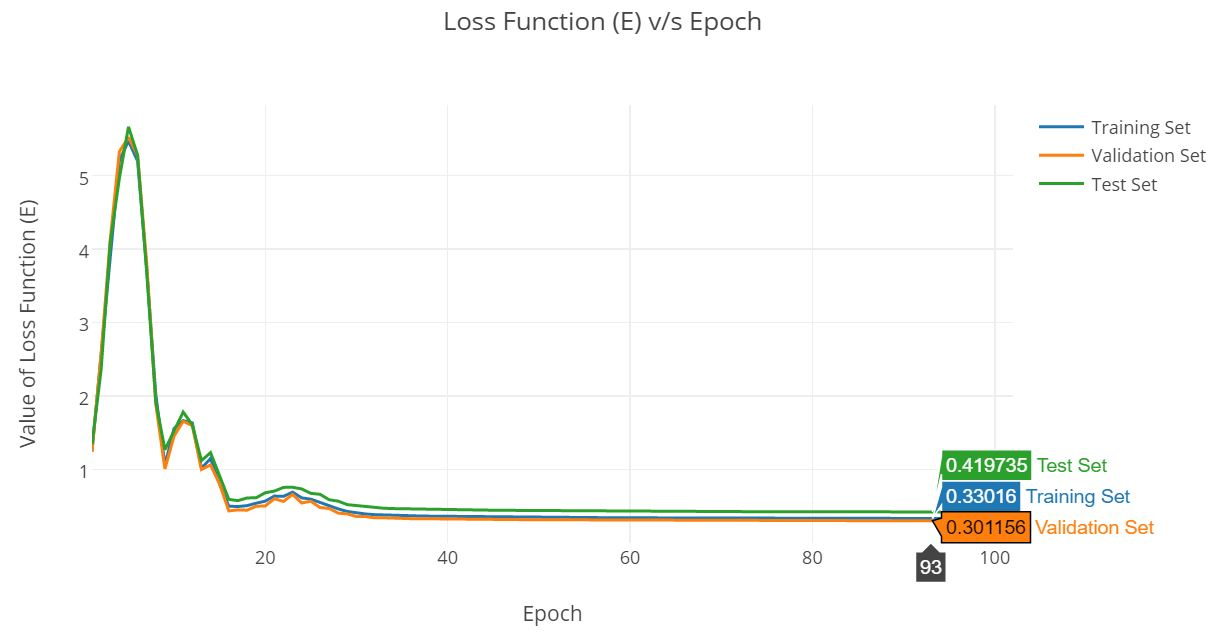
\includegraphics[width=120mm]{graphs/6b_softmaxLossVsEpoch.JPG}
  \caption{Loss Function(E) v/s Epoch}
  \label{fig:graph 6(b)}
\end{figure}

\begin{figure}[h!]
  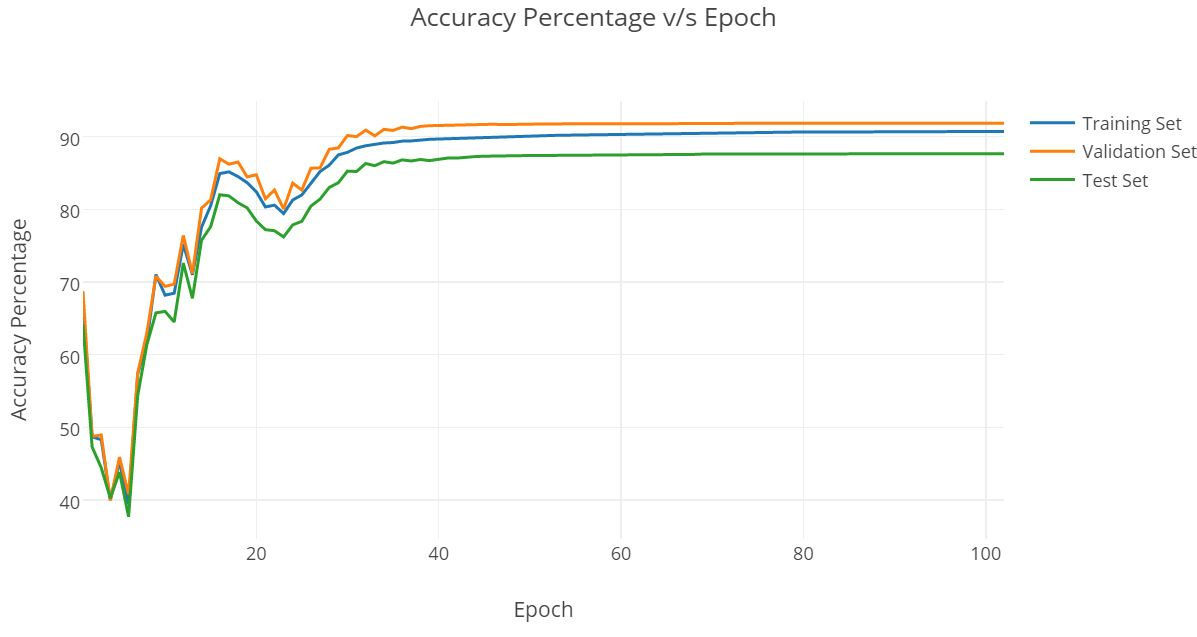
\includegraphics[width=120mm]{graphs/6c_softmaxAccuracyVsEpoch.JPG}
  \caption{Accuracy Percentage v/s Epoch}
  \label{fig:graph 6(c)}
\end{figure}


\subsection{Discussion}

As evident from the given table, the optimum value of error on hold-out (validation) set was obtained at more than one pair of values of $\eta$ and $\lambda$. We decided to go with the highest $\eta$ and the largest non-zero $\lambda$ that gave us the optimum error value on hold-out set. This is because we wanted $\lambda$ as large as possible to help generalization and avoid over-fitting, and at the same time being a good representative of the data. Also, higher learning rate was preferred for faster convergence. Since the penalties at both $L_{2}$ and $L_{1}$ norm did not seem to affect the error values, we decided to go forward with $L_{2}$ norm, as it gives a better measure of loss and is convex everywhere.

Thus, the hyper-parameters chosen were":
Penalty = $L_{2}$ norm
Regularization parameter $\lambda$ = 0.1
Learning rate $\eta$ = 0.0001

Validation Error = 8.1%

Test Error obtained = 12.35%

Note that early stopping was used to make sure that we do not over-fit the data.
 
Graph \ref{fig:graph 6(b)} shows how the training, validation and test errors vary according to the iteration number (epoch) for the same values of hyper-parameters. As evident from the graph, the loss function decreases and stabilizes over time, which corresponds to convergence. As an indicative measure, the values of test, validation and training errors have been displayed for a particular value (93) of epoch.

Graph \ref{fig:graph 6(c)} shows how the training, validation and test percent correct values vary according to the iteration number (epoch) for the same values of hyper-parameters. As evident from the graph, the accuracy saturates over time and does not improve. The weights learned give the best performance on validation set, followed by training and test set. It is interesting to note that all the values are fairly close to each other and similar in shape, which means that the training set is a good representative of the hold-out and test sets.


\newpage
\section{Results and Learnings}
The best accuracy achieved using Logistic Regression was more than 97\% for both the subsets of data - having digits 2 and 3, and having digits 2 and 8. The best learning rate was $\eta$ = 0.0001 and the best regularization parameter $\lambda$ was 0.0001 for 2’s and 3’s, and 0.1 for 2’s and 8’s. Using Softmax Regression, our accuracy was around 87.65\% on test data. The $\lambda$ used in this case was 0.001 while the learning rate was kept to be 0.0001. Annealing of learning rate per iteration helped us avoid over-fitting of the data, even when number of iterations was huge. This annealing parameter was set to a convenient value (2000) to ensure a gradual yet sufficient decrease in learning rate. The early stopping margin for number of iterations was set to 15 for the both the cases to ensure that the algorithm was not stopping at some sub-optimal value, which was the case when this value was small.

Having taken courses like 250A and 250B, we knew the working and mechanism of Logistic and Softmax Regression, but we had never had a chance to perform their in-depth analysis by ourselves. Deriving the expressions and implementing these two algorithms along with regularization gave us a new insight and deep understanding of the working of these methods. Questions involving plotting of loss functions, weight vectors as images and weight vector lengths showed us how these values vary with different regularization parameters $\lambda$ and the iteration number. We had never looked at the MNIST digit classification problem from this perspective and now have a clearer idea as to how the various hyper-parameters are related to each other. The impact of regularization on the model and weights is now in front of us, while previously we only looked at it theoretically. The concepts of annealing and early stopping were entirely new to us, as these concepts were never visible when using \emph{scikit} for performing these computations.
\section{Individual Contributions}
Being roommates, it was extremely convenient and simple for both the authors to coordinate and work in sync, while ensuring equal distribution of work and time spent on the assignment. Whenever one of the authors got stuck at some point, the other was there to help him out and unblock instantly. The process was initially started with both of us sitting down and solving on a white board the various derivations involved. The work thereafter was taken up as under:

Chetan Gandotra implemented the part which involved reading of MNIST data and implemented Softmax Regression. Then, debugging and graph plotting of Logistic Regression was taken up by him.

Rishabh Misra took up the implementation of Logistic Regression after extracting digit specific data. Thereafter, debugging and graph plotting of Softmax Regression was taken up by him.

The implementation and graphs for regularization question (Q5) were divided equally, with 5 (b) and 5 (c) being taken up by Chetan, and the others by Rishabh. For parameter tuning (values of $\lambda$, $\eta$, T, early stopping iteration number etc.), we made an Excel sheet with possible list of values and divided them equally amongst us. We then ran the code for these values for parameters on our respective systems.
When it came to writing the report, we took alternate question parts, with Rishabh taking odd questions and Chetan taking up even questions.

\newpage
\section*{References}

\small

[1] https://github.com/akosiorek/CSE/tree/master/MLCV

\section*{Appendix}

LoadMNIST.py
\begin{lstlisting}
import os, struct
from array import array as pyarray 
from numpy import append, array, int8, uint8, zeros

def load_mnist(dataset="training", digits=None, path=None, asbytes=False, selection=None, return_labels=True, return_indices=False):
    """
    Loads MNIST files into a 3D numpy array.

    You have to download the data separately from [MNIST]_. It is recommended
    to set the environment variable ``MNIST`` to point to the folder where you
    put the data, so that you don't have to select path. On a Linux+bash setup,
    this is done by adding the following to your ``.bashrc``::

        export MNIST=/path/to/mnist

    Parameters
    ----------
    dataset : str 
        Either "training" or "testing", depending on which dataset you want to
        load. 
    digits : list 
        Integer list of digits to load. The entire database is loaded if set to
        ``None``. Default is ``None``.
    path : str 
        Path to your MNIST datafiles. The default is ``None``, which will try
        to take the path from your environment variable ``MNIST``. The data can
        be downloaded from http://yann.lecun.com/exdb/mnist/.
    asbytes : bool
        If True, returns data as ``numpy.uint8`` in [0, 255] as opposed to
        ``numpy.float64`` in [0.0, 1.0].
    selection : slice
        Using a `slice` object, specify what subset of the dataset to load. An
        example is ``slice(0, 20, 2)``, which would load every other digit
        until--but not including--the twentieth.
    return_labels : bool
        Specify whether or not labels should be returned. This is also a speed
        performance if digits are not specified, since then the labels file
        does not need to be read at all.
    return_indicies : bool
        Specify whether or not to return the MNIST indices that were fetched.
        This is valuable only if digits is specified, because in that case it
        can be valuable to know how far
        in the database it reached.

    Returns
    -------
    images : ndarray
        Image data of shape ``(N, rows, cols)``, where ``N`` is the number of images. If neither labels nor inices are returned, then this is returned directly, and not inside a 1-sized tuple.
    labels : ndarray
        Array of size ``N`` describing the labels. Returned only if ``return_labels`` is `True`, which is default.
    indices : ndarray
        The indices in the database that were returned.

    Examples
    --------
    Assuming that you have downloaded the MNIST database and set the
    environment variable ``$MNIST`` point to the folder, this will load all
    images and labels from the training set:

    >>> images, labels = ag.io.load_mnist('training') # doctest: +SKIP

    Load 100 sevens from the testing set:    

    >>> sevens = ag.io.load_mnist('testing', digits=[7], selection=slice(0, 100), return_labels=False) # doctest: +SKIP

    """

    # The files are assumed to have these names and should be found in 'path'
    files = {
        'training': ('train-images.idx3-ubyte', 'train-labels.idx1-ubyte'),
        'testing': ('t10k-images.idx3-ubyte', 't10k-labels.idx1-ubyte'),
    }

    if path is None:
        try:
            path = 'C:\\Users\\Chetan\\Documents\\Python Scripts\\Way1'
            #path = os.environ['MNIST']
        except KeyError:
            raise ValueError("Unspecified path requires environment variable $MNIST to be set")

    try:
        images_fname = os.path.join(path, files[dataset][0])
        labels_fname = os.path.join(path, files[dataset][1])
    except KeyError:
        raise ValueError("Data set must be 'testing' or 'training'")

    # We can skip the labels file only if digits aren't specified and labels aren't asked for
    if return_labels or digits is not None:
        flbl = open(labels_fname, 'rb')
        magic_nr, size = struct.unpack(">II", flbl.read(8))
        labels_raw = pyarray("b", flbl.read())
        flbl.close()

    fimg = open(images_fname, 'rb')
    magic_nr, size, rows, cols = struct.unpack(">IIII", fimg.read(16))
    images_raw = pyarray("B", fimg.read())
    fimg.close()

    if digits:
        indices = [k for k in range(size) if labels_raw[k] in digits]
    else:
        indices = range(size)

    if selection:
        indices = indices[selection] 
    N = len(indices)

    images = zeros((N, rows, cols), dtype=uint8)

    if return_labels:
        labels = zeros((N), dtype=int8)
    for i, index in enumerate(indices):
        images[i] = array(images_raw[ indices[i]*rows*cols : (indices[i]+1)*rows*cols ]).reshape((rows, cols))
        if return_labels:
            labels[i] = labels_raw[indices[i]]

    if not asbytes:
        images = images.astype(float)/255.0

    ret = (images,)
    if return_labels:
        ret += (labels,)
    if return_indices:
        ret += (indices,)
    if len(ret) == 1:
        return ret[0] # Don't return a tuple of one
    else:
        return ret
\end{lstlisting}

Logistic_Regression_via_Gradient_Descent.py
\begin{lstlisting}
"""
CSE 253: Neural Networks and Pattern Recognition
Logistic Regression With and Without Gradient Descent
This file contains code for questions 4 and 5, including all graph plots
"""
import numpy
import math
import matplotlib.pyplot as plt
import plotly.plotly as py1
import plotly.graph_objs as go

from LoadMNIST import load_mnist
#----------------------------------------Utility functions--------------------------------------
def get_data(N, N_test):
    #load MNIST data using libraries available
    training_data, training_labels = load_mnist('training')    
    test_data, test_labels = load_mnist('testing')
    
    training_data = flatArray(N, 784, training_data) #training_data is N x 784 matrix
    training_labels = training_labels[:N]
    test_data = flatArray(N_test, 784, test_data)
    test_labels = test_labels[:N_test]

    # adding column of 1s for bias
    training_data = addOnesColAtStart(training_data)
    test_data = addOnesColAtStart(test_data)
    
    # Last 10% of training data size will be considered as the validation set
    N_validation = int (N / 10)
    validation_data = training_data[N-N_validation:N]
    validation_labels = training_labels[N-N_validation:N]
    N=N-N_validation
    #update training data to remove validation data
    training_data = training_data[:N]
    training_labels = training_labels[:N]    

    return training_data, training_labels, test_data, test_labels, validation_data, validation_labels
    
def flatArray(rows, cols, twoDArr):
    flattened_arr = numpy.zeros(shape=(rows, cols))
    for row in range(0, rows):
        i=0
        for element in twoDArr[row]:
            for el1 in element:
                flattened_arr[row][i] = el1            
                i = i+1
    return flattened_arr
    
def addOnesColAtStart(matrix):
    Ones = numpy.ones(len(matrix))
    newMatrix = numpy.c_[Ones, matrix]
    return newMatrix
    
# custom sigmoid function; if -x is too large, return value 0
def sigmoid(x):
    if(-x < 709):
        return 1 / (1 + math.exp(-x))
    else:
        return 1 / (1 + math.exp(708))

def extract_digit_specific_data(digits, data, label):
    pruned_data = numpy.zeros(shape = (1, len(data[0])))
    pruned_labels = []
    cnt = 0
    for i in range(0, len(label)):
        if label[i] in digits:
            if (cnt == 0):
                for j in range(len(data[0])):
                    pruned_data[0][j] = data[i][j]
            else:
                pruned_data = addRowToMatrix(pruned_data, data[i])
            pruned_labels.append(digits.get(label[i]))
            cnt = cnt + 1
    return pruned_data, pruned_labels
        
def addRowToMatrix(matrix, row):
    newMatrix = numpy.zeros(shape = ((len(matrix) + 1), len(matrix[0])))
    for i in range(len(matrix)):
        newMatrix[i] = matrix[i]
    newMatrix[i+1] = row
    return newMatrix
    
def calculate_log_liikelihood(data, label, weights, t):
    log_likelihood = 0.0
    for j in range(0,t):
        #print(numpy.log(sigmoid(numpy.dot(weights, data[j]))))
        log_likelihood += (label[j]*numpy.log(sigmoid(numpy.dot(weights, data[j])))) + ((1-label[j])*numpy.log(sigmoid(-1*numpy.dot(weights, data[j]))))
        
    return -1*log_likelihood/t

# 5.b, 5.c - Plot of Percent correct on training data v/s iterations, 
#length of weight vector v/s lambda
def plotlyGraphsRegularization(error_plot_array, lamda_vals, graph_name, min_index = -1):
    py1.sign_in('chetang', 'vil7vTAuCSWt2lEZvaH9')

    trace = []
    
    for i in range(len(lamda_vals)):
        y1 = error_plot_array[i]
        #y1 = y1[:min_index[i]]
        x1 = [j+1 for j in range(len(y1))]
        
        trace1 = go.Scatter(
            x=x1,
            y=y1,
            name = 'lambda = ' + (str)(lamda_vals[i]), # Style name/legend entry with html tags
            connectgaps=True
        )

        trace.append(trace1)
    data = trace

    fig = dict(data=data)
    py1.iplot(fig, filename=graph_name)
    
def plotlyGraphs(error_plot_array, labels, name):
    py1.sign_in('cgandotr', '3c9fho4498')
    trace = []
    
    for i in range(len(labels)):
        y1 = error_plot_array[i]
        y1 = [k for k in y1]
        x1 = [(j+1) for j in range(len(y1))]
        
        trace1 = go.Scatter(
            x=x1,
            y=y1,
            name = str(labels[i]), # Style name/legend entry with html tags
            connectgaps=True
        )
        trace.append(trace1)
    data = trace
    fig = dict(data=data)
    py1.iplot(fig, filename=name)
    
def early_stopping(early_stopping_horizon, accuracy, i):
    if i > early_stopping_horizon + 1:
        counter = 0;
        for p in range(0,early_stopping_horizon):
            if accuracy[i-p] <= accuracy[i-p-1]:
                counter+=1
            else:
                break
        
        if(counter == early_stopping_horizon):
            return True
        else:
            return False
            
def calculate_error(weights, data, label):
    error = 0.0;    
    for j in range(0,len(data)):
        prediction = sigmoid(numpy.dot(weights, data[j]))
        if(prediction>0.5 and label[j]!=1):
            error += 1;
        elif (prediction<=0.5 and label[j]!=0):
            error += 1;
    return error;
    
def dropFirstColumn(weights):
    return numpy.array(weights)[0][1:]

def fit(training_data, training_label, test_data, test_label, validation_data, 
        validation_label, digits, learning_rate=0.0001, iteration=200, batch_size=0, T=5000, lamda_vals=[0], norm=2):
    
    t = len(training_data)
    accuracy_plot_array = []
    log_likelihood_array = []
    weight_vector_length_array = []
    accuracy_plot_training_array = []
    weights_for_all_lamda = []
    test_error_array = []
    org_learning_rate = learning_rate
    
    for lamda in lamda_vals:
        weights = numpy.matrix(numpy.zeros(len(training_data[0])))
        weights_array = []
        weight_vector_length = []
        
        accuracy_plot_training = []
        accuracy_plot_validation = []
        accuracy_plot_testing = []
        
        log_likelihood_training = []
        log_likelihood_validation = []
        log_likelihood_testing = []
        min_error_index = 0
        learning_rate = org_learning_rate
    
        for i in range(0, iteration):
            # initialise Gradient
            gradient = numpy.matrix(numpy.zeros(len(training_data[0])))
            cnt = 0
        
            norm_term = []
            if (norm == 2):
                norm_term = l2_norm(lamda, weights)
            else:
                norm_term = l1_norm(lamda, weights)
                
            # calculate gradient over all the samples
            for j in range(0,t):
                # update gradient
                gradient += ((training_label[j]) - sigmoid(numpy.dot(weights, training_data[j])))*numpy.array(training_data[j])
                cnt += 1            
                if (batch_size != 0 and cnt == (int)(t/batch_size)):
                    cnt = 0
                    weight_vector_length.append(numpy.linalg.norm(weights))
                    weights = weights + learning_rate * (gradient - norm_term)
                    # re-initialise Gradient
                    gradient = numpy.matrix(numpy.zeros(len(training_data[0])))
                    # calculating log likelhood of training, validation and test dataset
                    log_likelihood_training.append(calculate_log_liikelihood(training_data, training_label, weights, t))
                    log_likelihood_validation.append(calculate_log_liikelihood(validation_data, validation_label, weights, len(validation_data)))
                    log_likelihood_testing.append(calculate_log_liikelihood(test_data, test_label, weights, len(test_data)))
        
            if (batch_size == 0):
                weight_vector_length.append(numpy.linalg.norm(weights))
                # update weights vector according to the update rule of Gradient descent method
                weights = weights + learning_rate * (gradient - norm_term)
                
                # calculating log likelhood of training, validation and test dataset
            log_likelihood_training.append(calculate_log_liikelihood(training_data, training_label, weights, t))
            log_likelihood_validation.append(calculate_log_liikelihood(validation_data, validation_label, weights, len(validation_data)))
            log_likelihood_testing.append(calculate_log_liikelihood(test_data, test_label, weights, len(test_data)))
                
            # anneling of learning rate
            learning_rate = learning_rate/(1+i/T)
        
            # calculating error percentage on train, test and validation data
            accuracy_plot_training.append((len(training_data) - calculate_error(weights, training_data, training_label))*100/len(training_data))
            accuracy_plot_validation.append((len(validation_data) - calculate_error(weights, validation_data, validation_label))*100/len(validation_data))
            accuracy_plot_testing.append((len(test_data) - calculate_error(weights, test_data, test_label))*100/len(test_data))

            weights_array.append(weights)        

            # check for early stopping
            early_stopping_horizon = 15
            min_error_index = i
            if(early_stopping(early_stopping_horizon, accuracy_plot_validation, i) and i > early_stopping_horizon):
                min_error_index = i-early_stopping_horizon;
                weights = weights_array[min_error_index]
                break
           
        weight_vector_length_array.append(weight_vector_length)
        weights_for_all_lamda.append(weights)
        
        log_likelihood_array.append(log_likelihood_training);
        log_likelihood_array.append(log_likelihood_validation);
        log_likelihood_array.append(log_likelihood_testing);
        accuracy_plot_array.append(accuracy_plot_training)
        accuracy_plot_array.append(accuracy_plot_validation)
        accuracy_plot_array.append(accuracy_plot_testing)  
        accuracy_plot_training_array.append(accuracy_plot_training)
        
        test_error = (calculate_error(weights, test_data, test_label)*100)/len(test_data)
        validation_error = (calculate_error(weights, validation_data, validation_label)*100)/len(validation_data)
        print('Error on validation dataset : ' + str(validation_error) + '%');
        print('Error on test dataset : ' + str(test_error) + '%');
        test_error_array.append(test_error)
    
    #For single lambda value
    if (len(lamda_vals) == 1):
        plotlyGraphs(log_likelihood_array, ['Training Set','Validation Set','Test Set'], 'Log Likelihood Plot')    
        plotlyGraphs(accuracy_plot_array, ['Training Set','Validation Set','Test Set'], 'Percent Correct Plot')    
    #else:
        #For multiple lambda values
        #plotlyGraphsRegularization(accuracy_plot_training_array, lamda_vals, "Accuracy vs Epoch")
        #plotlyGraphsRegularization(weight_vector_length_array, lamda_vals, "Weight Vector Length vs Epoch")
        #plotlyErrorVsLamda(test_error_array, lamda_vals)
    
    # printing error on training and testing dataset
    return weights_for_all_lamda
    
def plot_weights(weights):
    lamda_vals = [1000, 100, 10, 1, 0.1, 0.001, 0.0001]
    i = 0
    for w in weights:
        # Plot weights as image after removing bias terms. The rest of columns are pixels
        print ('lambda = ' + str(lamda_vals[i]))
        i += 1
        pixels1 = dropFirstColumn(w)
        pixels = numpy.reshape(pixels1, (28, 28))
        plt.imshow(pixels, cmap='gray')
        plt.show()    
    
def l2_norm(lamda, weights):
    return 2*lamda*weights;
    
def l1_norm(lamda, weights):
    w = numpy.ones(len(weights))
    for i in range(len(weights)):
        if (weights[i] < 0):        
            w[i] = -1
    return lamda*w;
    
# 5.d - Final test error v/s Lambda values graph
# Generates bar graphs
def plotlyErrorVsLamda(test_error_array, lamda_vals):
    lamda_vals1 = [math.log(lamda) for lamda in lamda_vals]
    py1.sign_in('chetang', 'vil7vTAuCSWt2lEZvaH9')
    trace = []
    colors = ['rgb(104,224,204)', 'rgb(204,204,204)', 'rgb(49,130,189)', 'rgb(41,180,129)']    
    for i in range(0, len(test_error_array)):
        y1 = test_error_array[i]
        x1 = lamda_vals1[i]
        
        trace1 = go.Bar(
            x=x1,
            y=y1,
            name='Lambda = log(' + (str)(lamda_vals[i]) + ')',
            marker=dict(
            color=colors[i]
            )
        )
        trace.append(trace1)
    
    layout = go.Layout(
        xaxis=dict(tickangle=-45),
        barmode='group',
    )
    fig = go.Figure(data=trace, layout=layout)
    py1.iplot(fig, filename='Final Error vs Lambda')
    
#---------------------------------------Main function------------------------------------------------------
        
if __name__ == "__main__":        
    numpy.random.seed(0)
    
    N = 20000
    N_test = 2000
    iteration = 200
    batch_size = 0
    T = 2000    
    
    #lamda_vals = [0]
    lamda_vals = [1000, 100, 10, 1, 0.1, 0.001, 0.0001] # regularization weightage parameter. Put [0] for no regularization
    norm = 2 # 2 for l-2 norm, 1 for l-1 norm
    
    full_training_data, full_training_label, full_test_data, full_test_label, full_validation_data, full_validation_label = get_data(N, N_test)
 
    # Parameters for training data on 2's and 3's
    digits = {2:1, 3:0}
    training_data, training_label = extract_digit_specific_data(digits, full_training_data, full_training_label)
    validation_data, validation_label = extract_digit_specific_data(digits, full_validation_data, full_validation_label)
    test_data, test_label = extract_digit_specific_data(digits, full_test_data, full_test_label)
    learning_rate = 0.0001 
    
    weights23 = fit(training_data, training_label, test_data, test_label, 
                    validation_data, validation_label, learning_rate, iteration, 
                    batch_size, digits, T, lamda_vals, norm)
    plot_weights(weights23)

    # Parameters for training data on 2's and 8's
    digits = {2:1, 8:0}
    training_data, training_label = extract_digit_specific_data(digits, full_training_data, full_training_label)
    validation_data, validation_label = extract_digit_specific_data(digits, full_validation_data, full_validation_label)
    test_data, test_label = extract_digit_specific_data(digits, full_test_data, full_test_label)
    learning_rate = 0.1 
    lamda_vals = [0] #Regularization not asked for with 2/8 case

    weights28 = fit(training_data, training_label, test_data, test_label, 
                    validation_data, validation_label, digits, learning_rate, iteration, 
                    batch_size, T, lamda_vals, norm)
    plot_weights(weights28)
    
    weights = weights28[0] - weights23[0]

    plot_weights(weights)
    
\end{lstlisting}

Softmax_Regression.py
\begin{lstlisting}
"""
Softmax Regression on MNIST Data set to perform 10-way classification
"""
import numpy
import math
import plotly.plotly as py1
import plotly.graph_objs as go

from LoadMNIST import load_mnist

#----------------------------------------Utility functions--------------------------------------
def get_data(N, N_test):
    #load MNIST data using libraries available
    training_data, training_labels = load_mnist('training')    
    test_data, test_labels = load_mnist('testing')
    
    training_data = flatArray(N, 784, training_data) #training_data is N x 784 matrix
    training_labels = training_labels[:N]
    test_data = flatArray(N_test, 784, test_data)
    test_labels = test_labels[:N_test]

    # adding column of 1s for bias
    training_data = addOnesColAtStart(training_data)
    test_data = addOnesColAtStart(test_data)
    
    # Last 10% of training data size will be considered as the validation set
    N_validation = int (N / 10)
    validation_data = training_data[N-N_validation:N]
    validation_labels = training_labels[N-N_validation:N]
    N=N-N_validation
    #update training data to remove validation data
    training_data = training_data[:N]
    training_labels = training_labels[:N]    

    return training_data, training_labels, test_data, test_labels, validation_data, validation_labels
    
def flatArray(rows, cols, twoDArr):
    flattened_arr = numpy.zeros(shape=(rows, cols))
    for row in range(0, rows):
        i=0
        for element in twoDArr[row]:
            for el1 in element:
                flattened_arr[row][i] = el1            
                i = i+1
    return flattened_arr
    
def addOnesColAtStart(matrix):
    Ones = numpy.ones(len(matrix))
    newMatrix = numpy.c_[Ones, matrix]
    return newMatrix
    
# custom sigmoid function; if -x is too large, return value 0
def exp(x):
    if(x < 709):
        return math.exp(x)
    else:
        return math.exp(709)
        
def addRowToMatrix(matrix, row):
    newMatrix = numpy.zeros(shape = ((len(matrix) + 1), len(matrix[0])))
    for i in range(len(matrix)):
        newMatrix[i] = matrix[i]
    newMatrix[i+1] = row
    return newMatrix
    
def l2_norm(lamda, weights):
    return 2*lamda*weights;
    
def l1_norm(lamda, weights):
    w = numpy.ones((len(numpy.array(weights)), len(numpy.array(weights)[0])))
    for i in range(len(w)):
        for j in range(len(w[0])):
            if (weights[i,j] < 0):        
                w[i][j] = -1
    return lamda*numpy.matrix(w);

# custom sigmoid function; if -x is too large, return value 0
def sigmoid(x):
    if(-x < 709):
        return 1 / (1 + math.exp(-x))
    else:
        return 1 / (1 + math.exp(708))
    
def calculate_log_liikelihood(data, label, weights, t):
    log_likelihood = 0.0
    for j in range(0,t):
        log_likelihood += (label[j]*numpy.log(sigmoid(numpy.dot(weights, data[j])))) + ((1-label[j])*numpy.log(sigmoid(-1*numpy.dot(weights, data[j]))))
        
    return -1*log_likelihood/t
    
def plotlyGraphs(error_plot_array, labels, name):
    py1.sign_in('cgandotr', '3c9fho4498')
    trace = []
    for i in range(len(labels)):
        y1 = error_plot_array[i]
        y1 = [k for k in y1]
        #y1 = y1[:min_index[i]]
        x1 = [(j+1) for j in range(len(y1))]
        
        trace1 = go.Scatter(
            x=x1,
            y=y1,
            name = str(labels[i]), # Style name/legend entry with html tags
            connectgaps=True
        )

        trace.append(trace1)
    data = trace
    fig = dict(data=data)
    py1.iplot(fig, filename=name)
    
def early_stopping(early_stopping_horizon, accuracy, i):
    if i > early_stopping_horizon:
        counter = 0;
        for p in range(0,early_stopping_horizon):
            if accuracy[i-p] <= accuracy[i-p-1]:
                counter+=1
            else:
                break
        
        if(counter == early_stopping_horizon):
            return True
        else:
            return False
            
def calculate_error(weights, data, label, k = 10):
    error = 0.0;    
    for j in range(0,len(data)):
        softmax_denom = 0.0
        softmax_num = numpy.zeros(k);
        for x in range(0,k):
            softmax_num[x] = exp(numpy.dot(numpy.transpose(weights[:,x]), data[j]))
            softmax_denom += softmax_num[x]

        prediction = numpy.argmax(softmax_num/softmax_denom)
        if(prediction != label[j]):
            error += 1;
    return error;

def softmax_loss(weights, labels, data, c):
    loss = 0.0
    for i in range(len(data)):    
        softmax_denom = 0.0
        softmax_num = numpy.zeros(c);
        for x in range(0,c):
            softmax_num[x] = exp(numpy.dot(numpy.transpose(weights[:,x]), data[i]))
            softmax_denom += softmax_num[x]
        softmax = softmax_num[labels[i]]/softmax_denom
        if (softmax > 0):
            log_softmax = math.log(softmax)
        else:
            log_softmax = 0
        loss += (log_softmax)
    return -1*loss/(len(data))
    
def getSoftmax(k, weights, training_data, j):
    softmax_denom = 0.0
    softmax_num = numpy.zeros(k);
    for x in range(0,k):
        softmax_num[x] = exp(numpy.dot(numpy.transpose(weights[:,x]), training_data[j]))
        softmax_denom += softmax_num[x]
    return softmax_num/softmax_denom

def fit(training_data, training_label, test_data, test_label, validation_data, 
        validation_label, iteration = 1000, T=2000, lamda=0.001, 
        learning_rate = 0.0001, norm = 2):
    k = len(numpy.unique(training_label))
    t = len(training_data)
    weights = numpy.matrix(numpy.zeros((len(training_data[0]), k)))
    weights_array = []
        
    early_stopping_horizon = 15    
    error_plot = numpy.zeros(iteration)
    min_error_index = 0
    loss_array = []
    loss_training = []
    loss_validation = []
    loss_testing = []
    
    accuracy_plot_array = []
    accuracy_plot_training = []
    accuracy_plot_validation = []
    accuracy_plot_testing = []    
    test_error = 0.0    
    
    for i in range(0, iteration):
        # initialise Gradient
        gradient = numpy.matrix(numpy.zeros((len(training_data[0]), k)))
        
        # calculate gradient over all the samples
        for j in range(0,t):
            modified_label = numpy.zeros(k);
            modified_label[training_label[j]] = 1
            softmax = getSoftmax(k, weights, training_data, j)
            gradient += numpy.transpose(numpy.transpose(numpy.matrix(modified_label - softmax)) * numpy.matrix(training_data[j]))
        
        norm_term = 0.0
        if (norm == 2):
            norm_term = l2_norm(lamda, weights)
        else:
            norm_term = l1_norm(lamda, weights)
        # update weights vector according to the update rule of Gradient descent method
        weights = weights + learning_rate * (gradient  - norm_term)
        
        loss_training.append(softmax_loss(weights, training_label, training_data, k))        
        loss_validation.append(softmax_loss(weights, validation_label, validation_data, k))
        loss_testing.append(softmax_loss(weights, test_label, test_data, k))
        
        # calculating error percentage on train, test and validation data
        training_error = calculate_error(weights, training_data, training_label)
        validation_error = calculate_error(weights, validation_data, validation_label)
        test_error = calculate_error(weights, test_data, test_label)
        
        accuracy_plot_training.append((len(training_data) - training_error)*100/len(training_data))
        accuracy_plot_validation.append((len(validation_data) - validation_error)*100/len(validation_data))
        accuracy_plot_testing.append((len(test_data) - test_error)*100/len(test_data))
        
        learning_rate = learning_rate/(1+i/T)
        
        error_plot[i] = validation_error*100/len(validation_data);
        weights_array.append(weights)        

        # check for early stopping
        if (early_stopping(early_stopping_horizon, accuracy_plot_validation, i)):
            min_error_index = i-early_stopping_horizon;
            weights = weights_array[min_error_index]            
            break
        min_error_index = i
        
    loss_array.append(loss_training)
    loss_array.append(loss_validation)
    loss_array.append(loss_testing)
        
    accuracy_plot_array.append(accuracy_plot_training)
    accuracy_plot_array.append(accuracy_plot_validation)
    accuracy_plot_array.append(accuracy_plot_testing)
    
    # printing error on training and testing dataset
    print('Error on validation dataset : ' + str(error_plot[min_error_index]) + '%');
    print('Error on test dataset : ' + str(test_error*100/len(test_data)) + '%');

    return weights, loss_array, accuracy_plot_array
    
#---------------------------------------Main function------------------------------------------------------

if __name__ == "__main__":        
    numpy.random.seed(0)
    learning_rate = 0.0001
    N = 20000
    N_test = 2000
    lamda = 0.001       # regularization weightage parameter
    T = 2000
    iteration = 1000
    training_data, training_label, test_data, test_label, validation_data, validation_label = get_data(N, N_test)
    
    weights, loss_array, accuracy_plot_array = fit(training_data, training_label, 
                                                    test_data, test_label, validation_data, 
                                                    validation_label)    
    
    plotlyGraphs(loss_array, ['Training Set','Validation Set','Test Set'], "Loss Function and Iterations")
    plotlyGraphs(accuracy_plot_array, ['Training Set','Validation Set','Test Set'], "Accuracy and Iterations")
    
\end{lstlisting}
\end{document}
